
\chapter{Redax}

This chapter is all about the intricacies and nuances of the readout software.
If you aren't particularly experienced with c++, you're probably going to get mired in details.
If the difference to you between l-value reference and r-value reference is only one letter, and you don't understand the nuance of \texttt{std::move}, much of this chapter will be casting pearls.

At its core, redax doesn't do much: read data from digitizers, transform from CAEN format to strax format, compress, and write to disk.
It also has to collect metadata for front-end reporting, monitor digitizers for the general health of the readout, deal with configuration options and board programming, and all the other stuff that often slips through the cracks.
The devil, as always, is in the details.
This chapter will subdivide into the various different parts of redax, but first we must introduce the various base classes redax uses before diving into greater depth.

\paragraph{MongoLog}

This is the logging class.
A single instance of this is created at program start, and pointers to it are farmed out to everything that needs to log stuff (ie, pretty much everything).
Messages of \texttt{DEBUG} or lower are printed to screen and written to disk, while higher-level messages are also put into the database.
This class handles daily rotation of logfiles and the removal of the appropriate week-old file (or whatever value is specified for the log retention).
Note, it doesn't do a particularly fancy job of handling leap years.
This will break whenever the usual N mod 4 doesn't work, but this won't be until long after I've left.

\paragraph{Options}

Pretty much what it says on the tin.
This pulls the various subconfigs from the database and assembles them into one, and provides an interface for the rest of the program to access values.
Also, because reasons, handles the storing of the baseline parameters and performance measurements.
One of these classes is instantiated when an ARM command is received, and it is destroyed on STOP.

\paragraph{DAQController}

This class is the one-off class that does all the high-level operations.
It owns the objects representing the boards, the majority of the threads, and is what \texttt{main} interfaces with via functions like \texttt{Arm}, or \texttt{Start}, etc.
Also, because reasons, this class implements the function that puts status update documents into the database.
The crate controller is a subclass of this.

\paragraph{V1724}

This is the primary digitizer class, handling pretty much everything digitizer-specific.
Subclasses at time of writing include the V1724\_MV for the muon veto, the V1730 for the neutron veto, and the f1724 for the waveform simulator.

\section{Executable}

Earlier versions of redax had two executables, a \texttt{main} for reading data from digitizers, and a \texttt{ccontrol} for the crate controller.
There's nothing inherently wrong with this, but it means that the \texttt{main} function is implemented twice and is effectively identical.
If you having the crate controller subclass the DAQController base, you only need to add one extra CLA, and the executables can be the same.
This simplifies the Makefile and the program usage.

The control flow for \texttt{main} isn't complex.
It starts with the usual creation of your main objects (or the pointers to the same), checks a few things, and enters the main loop.
The main loop pings the db for new commands, handles them, and then sleeps for \SI{100}{\milli\second}, until told to stop.
\texttt{main} also owns the thread that does the status reporting, more on this later.
When an ARM command is received, it creates an Options object with the specified config name, and then passes this to the DAQController instance via the \texttt{Arm} function.
If this returns successfully, the arming sequence is completed and the system can receive a STOP or START command.
The START and STOP commands do exactly that, with the STOP also deleting the Options instance.
The loop continues until it crashes, or a QUIT command is received.
Threads are then closed, objects garbage collected, and the program returns.

Earlier in the release schedule (back when there were two exes), the arguments were strictly positional.
The first argument was the ID number, the second was the database URI, and the third was (optionally) the name of the database to use.
I'm not the best at using \texttt{getopt\_long} so there are one or two known issues I couldn't be bothered to fix.
Specifically, if you specify a non-existent option, you segfault.
Submit a PR it it means so much to you.

Other options added rather later allow you to specify where you want the logs written and how many days you want logfiles kept around for.

There's also simple support for catching \texttt{SIGINT}s and \texttt{SIGTERM}s, but gdb does this itself so that code won't get used ever.

\subsection{Status reporting}

Originally, the DAQController class provided a few functions that returned the information needed for readers to post status updates, and the CControlHandler class just returned a document.
This second option is something that actually provides viable subclass implementation, as the crate controller doesn't post the same kind of documents as readers.
However, this means that the DAQController needs to know about the Mongocxx types, which means more \texttt{\#include} statements and a larger object file size.
This does enable the status reporting function to just call this one function and receive back the document that it will insert, rather than call several interface functions and assemble the document itself.
There are two options here: either \texttt{DAQController::StatusUpdate} has to return a document, or take a pointer to the collection as an argument.
I chose the latter, not entirely sure it was the best, but the argument really nickel-and-dimes so it's unlikely that it'll ever matter.

\section{MongoLog}

Logging is always very important for any software package that's larger than about 20 lines.
This class has three ``significant'' functions and a handful of shorter routines.
The constructor just starts a thread and opens its own connection to the database.
Most of \texttt{MongoLog::RotateLogFile} handles figuring out the filename of last week's log so it can get deleted.
\texttt{MongoLog::Entry} first assembles the variable-length argument list into one string, then pushes this full message into a queue.
Neither \texttt{stdout}, file, nor the Mongo collection are thread-safe, so everything pushes messages into a queue, and one thread handles things in the queue.
This is one reason why one instance of the class is made and pointers distributed.
The message is then printed to console, the logfile rotated (if necessary) before the message is written there, and (if the log level is sufficiently high) a document is made and inserted.
The remaining functions handle ensuring a common and consistent date format (\texttt{\%F \%T}), turning a \texttt{struct tm*} into a YYMMDD int, and generating logfile names from \texttt{struct tm*} objects.

\subsection{nT-style logging}

We made a specific subclass for nT-compliant logging using the specified storage structure.
It isn't fancy, but it's an example of what can be done.

\paragraph{Rant on message formatting}
The prefix-\texttt{printf} function that handles variable-length output to a buffer is \texttt{vsnprintf}, taking as arguments the output buffer, number of characters to write, format, and argument list, and returning the number of characters written.
This means to properly format the message, you must first call \texttt{vsnprintf} to find out how many characters you need (ie, what size buffer do you allocate), then create a \texttt{std::string} with this length (plus one because null byte), then call \texttt{vsnprintf} again and have it write to your vector.
C++20 has some nice new string-formatting, but we can't get these from Ubuntu 18.04, and the CAEN A3818 driver is only compatible with kernel major version 4 (note that this changed relatively recently but we'd have to update to 20.04 and that's a bit of a major thing).
This rant used to be much longer, but newer c++ standards changed \texttt{std::string::data} from a \texttt{const char*} to a \texttt{char*}, which eliminated the need for an intermediate \texttt{std::vector<char>} and an associated allocation and copy step.

\paragraph{Rant on c-style date and time formatting}

C++20 has some nice new date-time objects, but we can't get these.
This needs the gcc version that ships with Ubuntu 20+, we still have 18.04.
Instead we're stuck with the \texttt{struct tm}, which doesn't have options for millisecond-precision or better.
There is a workaround, where you can create a \texttt{struct tm} from a \texttt{std::chrono::system\_clock::time\_point} that you created with whatever precision you want, but it's still a workaround.

\section{Options}

In all the DAQ programs I've worked with, the part that handles the options always seems to be unreasonably large.
The header file here defines six classes, one actual Options class and five simpler structs to support specific types and values that should be grouped together (like board definitions or crate controller settings).
Most unfortunately have mixed type, so a strict \texttt{std::map} isn't available, but \texttt{std::map<std::string, std::any>} technically would be.
This would simplify most things greatly.
{\em Mental note: do this.}

The interface exposed by the class has predictable things like \texttt{Options::GetInt}, \texttt{Options::GetLongInt}, \texttt{Options::GetString}, and \texttt{Options::GetDouble}, which do (nearly) exactly what they say on the tin.
The exception being Long and Double, because if a number would fit into an int, many drivers won't encode it as a long.
Also, some drivers convert longs to doubles, because (I assume) fuck you.
The average IEEE-conforming double does have 53 bits of integer precision, but it's still an unwanted type-cast that we now have to deal with.
The case is similar for doubles - if a driver decides that it can encode some value as an int, it'll do so.

\texttt{Options::GetNestedInt} is effectively a wrapper to \texttt{Options::GetInt} that splits the input path into substrings though a routine that demonstrates why string-handling in C is still frustrating.

Then there are a number of functions written to handle the grouped types, all of which have some or other nuance.
\texttt{Options::GetBoards} has to be able to handle all digitizers, so ``V17xx'' means any currently-supported board.
The crate controller, logic module, and HEV have nothing special about them here.
The \texttt{Options::GetCrateOpt} and \texttt{Options::GetHEVOpt} pull a variety of fields from the config doc, and if any one of them is either missing or the wrong type or something, the whole op fails, though \texttt{Options::GetCrateOpt} does support both integer and floating point values for the pulser frequency. This function also gives defaults of all values to 0, so if the config is bad you'll only find out because your system doesn't work as expected.

\texttt{Options::GetRegisters} isn't very complex, but it does support an option to require exact matches with the board serial number, because \texttt{board=='all'} may work for writes going to digitizers, but you only want very specific writes to happen to your logic module.

\texttt{Options::GetThresholds} does what it says on the tin. If it can't find the requested board in the map it returns a 16-element vector filled with \texttt{0xA}. \texttt{GetDAC} is similar, except it allows you to specify both how many and what default value to use in this case.

\texttt{Options::UpdateDAC} is called once per host after fitting the baselines and upserts into the database with this run's DAC values. \texttt{GetDAC} pulls the most recent document for the requested board and unpacks it.

\texttt{Options::GetV1495Opts} is an example of what I would liked to have done for several other functions, which just loads a \texttt{std::map<std::string, int>} with whatever you've specified in the config, without requiring you to have pre-specified specific fields.
Hopefully this means that you don't need to make pull requests to fix typos, you only need to fix your config.

\subsection{Rant}

The Mongocxx driver has some serious usability issues.
There's no \texttt{operator=}, so you can't modify a document once it's been created.
This makes assembling half a dozen documents into one rather frustrating.
There is a \texttt{concatenate\_doc} that can be used, but it's not particularly nice.
It doesn't replace fields, it just adds them, so you can get multiple fields with the same key and you only hope that the correct one is found when you request it.
Given that the \texttt{Options::Override} method is how the config is built (including any override options), if you have an option specified in both the ``proper'' document and the override, you're only most likely to get the correct one.
This can be done via an aggregate call, but it doesn't change the fact that the driver doesn't offer a lot of the tools that would make life easier.
Also sometimes documents don't get translated properly, so when you try to convert an array from the document into a \texttt{std::vector} occasionally the vector ends up empty and you segfault for no fault of your own.
It's also next to impossible to trace this back to its source and patch the problem out.

\section{V1724}

This class provides both the external interface for the DAQController object, and also the internal interface necessary so subclasses don't have to do that much.
A virtual function is provided for the board initialization, which will generally mean calling some CAEN library functions, maybe setting a few runtime variables, etc.
This function gets called by the constructor, which is at the beginning of the arming sequence.
Most of what the constructor does is setting the register values and a couple of model-specific parameters like channel count, sample rate, etc.
The V1724 class doesn't own an instance of Options, because once the initialization sequence is finished it never needs to refer to it.

A variety of interface functions are provided for the owning DAQController.
These are functions like \texttt{V1724::SINStart}, \texttt{V1724::SoftwareStart}, \texttt{V1724::EnsureReady}, etc.
Most of these read from or write to a single register, except the \texttt{V1724::Ensure*} methods, which will repeatedly check a given register until it has a desired value, or until some maximum number of tries is reached.

A few more private (protected, technically) methods exist for tracking clock rollovers.
\texttt{V1724::GetClockInfo} returns a tuple containing the first board header timestamp and the board's rollover counter.
Clock rollovers are tracked via the simple \texttt{this\_clock < last\_clock} with the added realtime check (see section~\ref{}).
I'm still not entirely sure the realtime check is the best thing, though.

\subsection{\texttt{V1724::Read}}

This function is where most of the action happens.
If the board has at least one event available (bit 0x8 of the acquisition status register), then block transfers of are made until the board is empty.
There's a lot of nuance in how large of a buffer to allocate.
The digitizer can't tell you how many events it has, only what the size of the first one is, so we don't know \emph{a priori} how much memory to allocate.
We could just allocate however much memory the digitizer has, but most of the time the board only has a single photon event, as shown in Figure~\ref{fig:digi_blt}.

\begin{figure}
  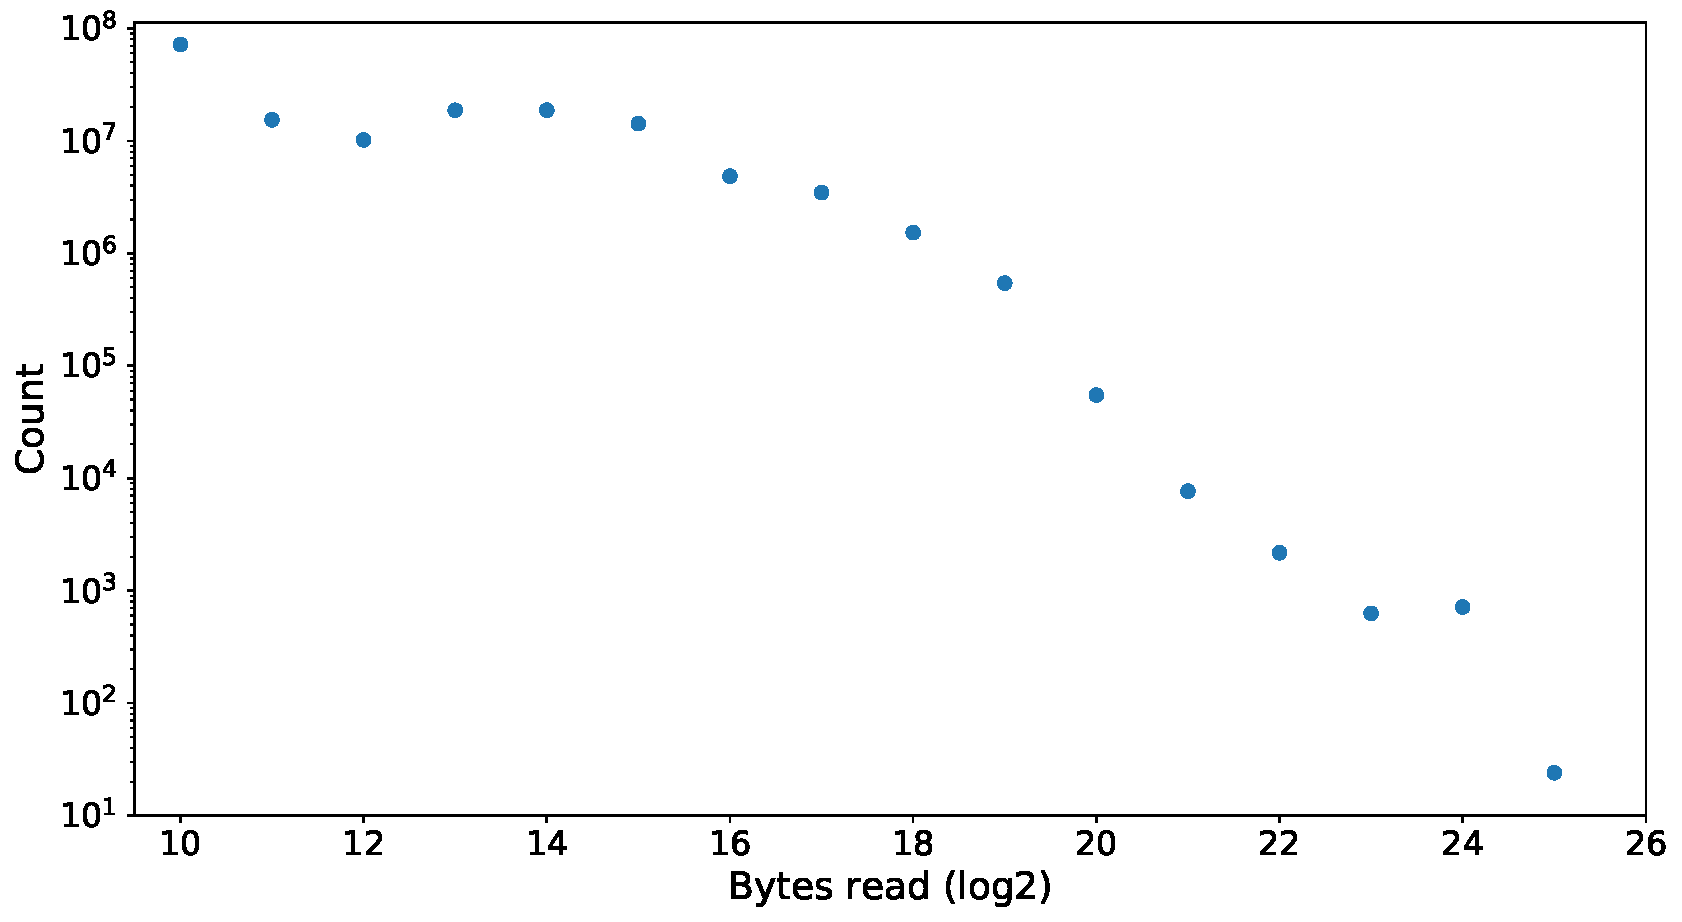
\includegraphics[width=\textwidth]{images/digi_blt}
  \caption{A histogram of the amount of data read out of a digitizer during background mode. A single photon waveform requires about 1~kB, and the digitizer only has 8~MB total storage. The events beyond 8~MB are from times when the digitizer records additional data while the readout is active.}\label{fig:digi_blt}
\end{figure}

Allocating on the heap is slow ($\mathcal{O}(\mathrm{\mu s})$), and allocating more memory takes more time.
It's a massive waste to ask for a buffer of 8~MB and then only put 1~kB into it.
However, if you start with a much smaller (and faster) allocation, what do you do if the board has more?
You could just allocate the same amount again, but unless you want to do a massive number of allocations you either have to start at the same order of magnitude as the total memory on the digitizer, or increase the allocation size each time.
The progression of size is something to optimize based on how fast a server allocates a given amount of memory, and how much memory needs allocation each time.
For the main TPC readers the optimal values (in $\log_2$) are \texttt{[16 19 20 23]}, and this cuts the time spent allocating memory in each run by half, which saves many minutes of CPU time.
If you get to the end of the sequence and there's still more data waiting, keep doubling the amount of memory you allocate and eventually you'll finish.

I spent a year trying to figure out how to get this optimization to actually work.
A naive implementation of this increasing buffer size doesn't work, because what if the first event is a massive honking S2 that won't fit into your initial allocation?
You crash is what happens, so despite a beautiful study we always have to allocate the full 8~MB.
Then I realized that the smart move would be to have the digitizer own a static readout buffer, rather than keep allocating readout buffers every single time a readout happens.
It's stupidly simple.

Also, the number of bytes requested from the digitizer is smaller than the buffer allocation by a factor of (by default) $1.5$, because sometimes you ask the driver for X bytes and you get more.
This can cause buffer overruns and memory-corruption crashes.
Once enough BLTs have happened, the buffers are concatenated into one, the rollovers are computed, and a \texttt{std::unique\_ptr<data\_packet>} is returned to the calling function (probably \texttt{DAQController::ReadLink}).

\subsubsection{Rant}

It's not efficient to do a bunch of small allocations into temporary locations and then one larger one to hold all of the smaller ones.
It would be really nice if the digitizer just told you how much memory it had buffered, rather than a yes-no, so we could always alloc exactly the right amount.
The alloc used to be done every time before checkint to see if the board had any data, but this is inefficient because most of the time the board doesn't have anything.
Further, the alloc size used to be the entire digitizer's memory (8~MB), but then certain unnamed persons who may or may not work on one of the veto readouts spent several minutes complaining that this buffer was too small and their readout wasn't working (the buffer may have been too small, but that isn't the reason why their readout wasn't working).
We then added this loop feature, which turned out to work pretty well.
We then removed this loop feature and went back to a single large buffer, but a bit smarter this time so it shouldn't cause the same kind of crashes as in the past.

And then when you start doing calibration at high-rates with very large (ie, wide) S2s, you'll end up in situations where the small allocation you make isn't nearly enough for the amount of data currently buffered in the digitizer.
The CAEN driver rounds up when you ask for data, so you ask for $2^{16}$ bytes, and it decides to give you $2^{21}$ or $2^{22}$ or something, because that's the next event in buffer.
You can't put a couple of megabytes into a 65~kB allocation, you'll overrun the buffer and die immeidately due to memory corruption.
This means that you can't do small allocations at all, so even if you only end up reading out a handful of single photons you still have to do a very large allocation because the driver might also give you a massive S2.

\subsection{Subclasses}

Initially the support for extra digitizers was handled through a truly terrible way where you'd specify \texttt{firmware\_version} in the config, and the data unpacking would proceed based on this value.
This was terrible and didn't work.
We then pivoted to use child classes, which was a good first step but with a mediocre implementation.
Each class and subclass would provide a map of values about how many words were in this header, indexes of where certain values were in these headers, etc, and the \texttt{StraxInserter} (the old name) had a bunch of \texttt{if}s to unpack things.
This was also terrible, so for the v2.0 release this was redone so that all digitizer-specific processing (unpacking headers) was handled by digitizer functions that a subclass could implement as necessary.
Now, the \texttt{StraxFormatter} just calls \texttt{V1724::UnpackEventHeader} and and \texttt{V1724::UnpackChannelHeader}, which lets the digitizer itself worry about which word means what.
It's beautiful.

\subsubsection{f1724}

The waveform simulator, aka fax, aka the fake V1724, is a testing tool.
It's implemented as a V1724 subclass so the rest of the system doesn't know the difference.
Most functions had to be rewritten for obvious reasons, and a significant number of extra members added.
For reference, the muon veto and V1730 subclasses are together about 3~kB in four files, while the waveform sim is larger than the V1724 base class itself.
For instance, the waveform sim needs a few objects for the random number generation, its own internal buffer with mutex and condition variable, vectors to store baseline and noise information, its own clock and event counters, and more.
On top of this, most of these are needed again at a global scope for the actual event generation.

\paragraph{Settings}

There are four (as of writing) configurable input options to the waveform sim:
\begin{enumerate}
  \item TPC size - this is given in units of PMT size. A value of 4 means the diameter is 9 PMTs (radius is 4, plus one in the middle) and the length is the same.
  \item Event rate - this is given in Hz.
  \item Drift speed - this is in units of PMTs/ns.
  \item Electron absorbtion length - this is in units of TPC lengths. Measuring electron livetime in units of time rather than distance is usually dumb.
\end{enumerate}

The TPC is assumed to be hexagonal and the PMTs arranged in identical hexagonal arrays, with each array containing $1+3\times size\times (size+1)$ numbered incrementally from the center and spiralling out.
Further, fax will automatically assume you have enough digitizers to ``read'' all of these, and you will segfault if your config doesn't match this.
PMTs are assigned to all channels 0, then channels 1, etc.

\paragraph{Simulation flow}

The simulation is divided into two separate phases.
The first is the actual ``physics'', which runs in a static thread.
There is only ever one of these, regardless of however many fake digitizers are created.
First, an event location is generated.
This is flat in theta, flat in depth with a minimum of 0.5, and also flat in radius (not radius squared).
Then, an S1 is generated between 11 and 30 photons.
The S2/S1 ratio is normally distributed with a mean at 100 and a width of 20, and the electron loss is $\exp depth/absorbtion$ (depth is generated as a negative number).
Once the S1 and S2 are generated, the hitpattern generation happens sequentially.
S1 width is 40ns (flat), and S2 width is $1000 + 200\sqrt{z}$ nanoseconds.
The top fraction is 65\% for S2s, and linear for S1s with 10\% at the bottom and 40\% at the top.
For S1s, PMTs in each array are treated equally.
For S2s, the top hitpattern is assumed to be Gaussian with a width of 1.3.
Finally, PMT hits are generated with the given time and spatial probabilities.

Once all the ``physics'' has finished, hits are divided according to their digitizer and sent to each individual fax instance for the actual waveform generation.
A baseline of noise is generated, and a single photon template waveform scaled, shifted, and added.
This is then converted to the digitizer format and added to the digitizer's buffer.
When \texttt{V1724::Read} is called, this buffer is \texttt{std::move}d into the data packet.

\paragraph{Things it doesn't do (yet)}

The trigger threshold is meaningless, pre- or post-trigger samples are based on the waveform template, and dark counts aren't a thing.
Dark counts probably can't be a thing without a total rewrite of the entire thing.

\section{DAQController}

This is the Highlander class of redax.
Only one instance is ever made, and it handles all of the fancy stuff.
This class owns all the digitizer instances, all the processor instances, etc.
\texttt{main} interfaces via clearly-purposed functions like \texttt{DAQController::Arm}, \texttt{DAQController::Start}, and \texttt{DAQController::Stop}.
They do exactly what they say on the tin, but it's certainly worth digging into how they're implemented.

\subsection{Arm}

This function is involved.
First, all digitizers assigned to this process are pulled from the config.
These are all initialized and assigned to \texttt{std::vector<std::shared\_ptr<V1724>>} based on their optical link.
Next, \texttt{sleep(2)}.
This is important, don't get rid of it.
Threads are now made for the parallel programming of digitizers.
This used to happen in serial, so it sometimes took quite a while, especially if the baselines were particularly noisy.

After programming, boards are put into a ``ready but not quite'' mode.
All main threads are now opened, first the processing threads and then the readout threads.
For what it's worth, there is a potential race around starting the boards, because two threads are trying to access various registers at the same time.
It hasn't caused any crashes after several thousand runs, though, so it isn't a common occurrence.
Still, this is a note that it should get fixed at some point.

\subsubsection{Programming and baselining}\label{sec:baseline}

The baselining has traditionally been a cause of some problematic behavior.
We'll go over this in chronological order, discussing the algorithms and why they were rewritten.
All versions follow the same overall flow, with the devil being in the details.
The sequence is as follows:
\begin{enumerate}
  \item Start boards via software
  \item Send SW triggers
  \item Stop boards via software
  \item Read everything out
  \item Calculate the baseline per channel
  \item Update the DC offset value based on the difference between the desired and actual values
  \item Repeat until ``done''
\end{enumerate}

\paragraph{Version 1}

The above sequence was followed with negligible delay between iterations.
Also, the baseline was calculated by averaging all the samples in each readout.
If the range of values exceeded some hard-coded value, the readout was rejected.
This algorithm had issues in converging, and also didn't work if the noise was particularly bad.

\paragraph{Version 2}

Somewhere in the CAEN docs it mentions that you should wait ``a few'' seconds after setting the DC offset, so the output can stabilize.
Version 1 didn't do this, so there were some convergence issues as there were usually a few iterations of delay between offset values being output and taking effect.
Eventually it all converged, but it would sometimes oscillate.
A value of \texttt{sleep(1)} was introduced, which largely eliminated this oscillation, and didn't actually impact the convergence time in any way.
Additionally, a number of key changes were introduced.
The approximate relationship between a difference in ADCs between desired and actual baseline, and the DC offset value is in principle known to be 0.25 (14-bit ADCs and 16-bit DAC), but the actual values wander considerably based on the production tolerances of the opamps and resistors.
These, in turn, depend on the board temperature.
A good idea is to first calibrate this relationship by outputting a few pre-defined DAC values, measuring the corresponding baseline, and fitting a line between them.
This means you don't need to shoot at random and hope you ended up ``close'' to the desired value, you can just consult the calibration.
Also, the slope of the line tells you how many DAC counts you need to change to effect the desired change in ADC counts.
The DAC values chosen were $60\,000$, $30\,000$, and $6000$, which cover most of the full range with an anchoring point near the ``expected'' value.

Further, the baseline was calculated by histogramming the waveform, which is much more resilient to random fluctuations, and also provides a variety of tools to rebin and reject outliers.
This proved to be particularly effective against all but the worst levels of noise, but still required all channels to converge to achieve ``convergence''.

\paragraph{Version 3}

The next logical progression is to allow individual channels to progress separately through the sequence, rather than requiring all channels to wait for the slowest.
When you get to the end of the sequence, you then treat any unconverged channels with some appropriate backup method.

\paragraph{Version 4}

I moved the function from \texttt{DAQController} to \texttt{V1724}.
This means it's very slightly slower because each steps are done in series rather than in parallel, but we're talking milliseconds here.
This change was largely done because certain unnamed people who may or may not work on the veto readouts were adamant that they didn't want the baseline routine done for their digitizers, and doing this allows them to implement the function to do nothing.
Also I got rid of the calibration step and put the calibration values into the config.
They vary between boards but are close enough that we can use one value and the function will handle it.

\subsection{Start}

This function does one of two things, depending on the value of \texttt{run\_start} in the config.
If the value is \texttt{0}, all digitizers are successively started via \texttt{V1724::SoftwareStart}.
If the value is \texttt{1}, all digitizers are successively started via \texttt{V1724::SINStart}.
Finally, the status variable is set to \texttt{Running}.

\subsection{Stop}

The first thing this function does is indicate to the readout threads that they should stop, and then it waits for up to a second for them to all return.
Next, all boards are put into the ``pre-ready'' mode (the S-IN signal usually is already low by this time).
If one board has crashed then usually an error message will be logged because that board isn't really responding normally.
Next, all the threads are stopped.
The mutex is locked, and the readout threads are joined first.
Processor threads are all stopped first, then all joined, and the objects garbage collected.
The digitizer objects are garbage collected, the run number reset, and the Options object destroyed.

\subsection{CC subclass}

A \texttt{DAQController} subclass was written as part of the executable unification.
It doesn't do anything fundamentally differently.

\section{StraxFormatter}

This is one of the other ``bulky'' classes, in terms of the amount of code it has.
Nothing is particularly fancy, but it's still worth talking about most of it.

\subsection{Flow}

\texttt{StraxFormatter::Process} is where most things revolve.
It's an infinite loop that sleeps as long as its internal buffer is empty.
When notified that data is awaiting processing, it moves data from its buffer into a temporary location (so the buffer mutex can be unlocked as soon as possible).
Then, it passes the \texttt{std::unique\_ptr<data\_packet>} to \texttt{StraxFormatter::ProcessDatapacket}.

Datapacket unpacking is as follows: words are looped over until an event-start signature is found.
This is then passed to \texttt{StraxFormatter::ProcessEvent}, along with the rest of the metadata from the data packet.
The return value of \texttt{ProcessEvent} is the number of words processed, and the pointer to the buffer is advanced by this amount.
Ideally, the next pointed-to word is another event start.
If this isn't the case, a message gets logged.
When the function returns, the datapacket (and its storage) is deallocated.

Event processing is as follows: first, the event header is unpacked via a call to \texttt{V1724::UnpackEventHeader}.
This returns the size of the event, the channel mask, the board failure status, and the timestamp of the event header.
If the board fail bit is set, this is propagated upstream and the remainder of the event discarded.
Otherwise, the pointer to the buffer is advanced, and channels are looped over.
If the i$^{th}$ channel is present in this event, \texttt{StraxFormatter::ProcessChannel} is called with the current location in the buffer and a bunch of metadata.

Channel processing is as follows: first, the channel header is unpacked via a call to \texttt{V1724::UnpackChannelHeader}.
This returns the global timestamp, the size of the payload, the baseline, and the actual waveform.
Then the global channel number is queried; if none is found this thread (and the rest of the process) kills itself.
Then, as many fragments as necessary are created and added to the chunk buffer.

The chunk number is found from the fragment timestamp, and the maximum and minimum currently-buffered chunk numbers are determined.
If the fragment in question is older than the minimum chunk by a configurable margin, a warning message is logged.
If the fragment is more than one chunk ahead of the buffer, a message is logged.
The fragment is then moved onto the buffer (implemented as a \texttt{std::list<std::string>}).

Once a data packet is processed, any applicable chunks (older than \texttt{average\_chunk - BufferNumChunks}) are written to disk, where the average is weighted by the number of fragments in each full chunk.
This helps protect against situations where one fragment somehow is ahead of the bulk of the buffer, and it causes everything else to get written out before its time.
A large enough buffer to store the full continuous chunk is allocated; the fragments are added to this, and then cleared.
An output buffer is allocated based on the compression algorithm, and the chunk is compressed into it.
The compressed output is written to a temporary file, and then moved to its non-temporary location.
If the output file already exists, a warning is logged before the file is overwritten.

Once all applicable chunks are written out, any previously skipped chunks are filled in with empty files.
For instance, if chunks 3 and 5 are written, but 4 was not because it didn't contain any data, an empty file is made in chunk 4's place, so the processing doesn't get held up.

\paragraph{Rant}

Why do fragments show up out of phase with the bulk?
I understand if we miss a rollover or accidentally accrue an extra, but a lot of times one channel will skip one chunk.

\section{V2718}

The crate controller handles all the five output control lines, including the external pulser.
Most of the code for this class is just programming the V2718 to set the desired outputs, but the frequency-determining block is worth discussing.

The pulser output does not support continuous frequencies.
It's implemented hardware-side by specifying a period unit (one of \SI{104}{\milli\second}, \SI{410}{\micro\second}, \SI{1.6}{\micro\second}, and \SI{25}{\nano\second}), and how many of them (1-255) specify the desired period of the output pulse.
This gives you access to both very low frequencies (\SI{38}{\milli\hertz}) and very high(\SI{40}{\mega\hertz}), and a variety in between.
The issue, however, is that there are often large gaps between available frequencies, and the chances are that you want to work in one of these gaps.
This is implemented by finding the smallest frequency that is larger than the value specified in the config file.

\paragraph{f2718}

It really does nothing, but the dispatcher assumes that crate controller executables are running, so it needed to exist.

\section{V1495}

The V1495 offers considerably more potential than we currently use.
This class used to exist purely to write a few registers, but it was redesigned to allow subclassing.
Four functions are provided for a subclass to implement, with any desired actions on either side of run start and stop.

\subsection{TPC subclass}

Initially the TPC V1495 was a ``dummy'' module that was never interfaced with unless new firmware needed loading.
However, with the introduction of the fractional livetime mode, it became necessary to write registers during programming.
This can be accomplished via entries in the general register list, but that only writes during the arming sequence.
No provision using this method exists for turing the fractional livetime mode off at the end of the run, and this caused some issues shortly after the introduction of this feature, because it was active when it wasn't supposed to be.
A subclass can turn the feature on when necessary at the start of a run, and then turn it off at the end.
Also, the subclass can hide the implentation details, and put convenient terms like \texttt{veto\_on\_us} in the config, rather than requiring a user to know that the value is a 32-bit number of 40~MHz clock cycles, split into two 16-bit integers.
This way, for the eventuality when the out-of-production V1495 is finally upgraded to the V2495, the configs don't need updating.

\section{DDC10}

This class doesn't do much.
It takes the provided options and passes them via ssh to the DDC10.
An option for the future is to ship a build of redax that can run natively on the DDC10, in which case this would be a new subclass of \texttt{DAQController}.

\section{Major bugs}

I won't cover any ``minor'' bugs here because I don't remember most of them, but we did have two ``major'' bugs during commissioning.

\subsection{Silent overwrites}

In the first few self-trigger runs after the TPC was connected, we realized that a lot of data was missing, and the pattern lined up very nicely with chunk boundaries.
The culprit was the logic surrounding when a buffered chunk was compressed and written to disk.
If you write out chunk N-1 as soon as the first fragment belonging to chunk N is seen, you had better hope that all the data in your buffer is time-ordered.
Hint: the buffer is only approximately time-ordered.
Also, there was no check to see if a chunk already existed when you were trying to write a chunk out.

The fix for this was two-fold.
First, buffer more than one chunk.
Second, throw a warning message if a chunk already exists.
A good idea would be to offer the option to append ``late'' fragments to an already-existing chunk, but this does cause some issues based on how far behind bootstrax is (usually, not very).

\subsection{Desync}

Part of the system synchronization requires that all digitizers receive and act on the S-IN signal at the same time.
However, if a digitizer sits around ready and waiting for the S-IN signal, and something that looks like an S-IN signal shows up briefly, you just threw off the clock rollover logic.
If one channel is taking a while to baseline, boards on other readers are going to be sitting around in this ready state for potentially a while.
The fix is to only put the boards into the fully readied state just in advance of the S-IN signal.
If git decides to screw you over based on the order in which you merge PRs, your carefully set delay between reader start (when the boards are readied) and CC start (when the S-IN signal shows up) gets undone.
This means that the time when the board is set to accept the S-IN is randomly distributed around the time when the S-IN signal is issued, rather than still being randomly distributed but guaranteed to be in advance of the S-IN signal itself.
If no one is really looking at data, it can take a while before anyone notices this.

This doesn't show up at anything less than the peak level.
All the pulses are still being recorded and written out so the overall data rate is unaffected, but their timestamp are now jumbled, so you'll only see this when you start looking at places where timestamps are important.
This is more or less fixable after the fact, but it's a bit of a hassle.

\section{Things we used to do}

Now, let's talk about the major design changes we've made over the development lifetime.

\subsection{Central data pipeline}

In much earlier versions of redax, readout threads would push data into one central buffer and processing threads would pull from it.
The form of this buffer changed over time, as did the nature of the pull.
Initially, the buffer was a \texttt{std::vector<std::vector<data\_packet*>>*}, and a processing thread would just pull the entire thing and start chewing on it.
For one, this is pretty poor design.
The push stage is relatively performant because you're just copying pointers, which doesn't take very long.
The pull stage is also performant because you're changing ownership of the pointer.
However, you can't load-balance, because then entire buffer goes to one thread.
If that buffer happens to be chunky, and the run nearly over, you might run into issues.
If the buffer is empty, the threads wait for a bit and then ask again.
A much better buffer is \texttt{std::list<data\_packet*>}, because adding and removing elements is constant-time at either end.
Maybe you use a managed rather than a raw pointer, but the point doesn't change.
Load-balancing is much easier, because you then give a requesting thread some fraction of the total number of things waiting for processing.
Still, it's better design for data to go via a push method in both ways, rather than push-pull.
Processing threads should sleep until notified that there's data waiting for them to handle.

What's even better, is to eliminate the central buffer entirely, and give each processing thread its own buffer.
This increases the number of available mutexes, which usually helps performance.
This also makes it easier to load-balance between the different processing threads, by having readout threads just cycle through which processing thread they're offloading data to.
If the processing threads operate via pull rather than push, it's possible for a thread to see no data for an entire run because it was particularly unlucky and the buffer was always empty when it asked for data.
This happened at least once.
With a push that cycles through all threads this becomes impossible.

\subsection{Chunk buffering}

How do you store a chunk while it's still being accumulated?
You can store it in a continuous block, but you don't know before-hand how large the chunk is going to be, so you're going to end up with $\log_2 size$ reallocations and copies as the chunk fills.
Or, you can store the fragments separately, only accumulating them into one continuous block once you're ready to write out.
The advantage here is that you now know exactly how many bytes to allocate, and only copy a given byte once.
A \texttt{std::list<std::string>} is a great way to implement this.

Also, what's the best way to handle the pre/post chunks?
You can associate them with the same full numbered chunk (N\_pre, N, N\_post), but this means you need extra logic to ensure that \texttt{000000\_pre} doesn't exist.
Alternately, you can associate them with discrete blocks of time (N, N\_post, N+1\_pre).
This has the added advantage that you don't need to buffer the overlap chunks twice, you buffer and compress once, and write out twice.

\section{Things that were never to be}

Let's talk about the major things I tried but couldn't get to work.

\subsection{One processing thread per digitizer}

This dated back to much earlier in our understanding of how best to handle clock rollovers in a multithreading environment.
What if you dedicate one thread to each digitizer's data?
This way, you don't have to worry about tracking rollovers in a thread-independent fashion.
However, this does have a few drawbacks.
First, a given board is always read out by the same thread, so having that thread also track rollovers isn't difficult.
Second, if a channel on one board starts shitting itself, its processing thread could start falling behind, and this causes issues if the run ends with a considerable amount of data still unprocessed.
If everything behaves like the average requires, this is fine, but PMTs flash, and it's really nice to distribute all that extra load over more than one thread.
Third, your readout server might not have that many threads.
The MV's server only has 8, and it uses 3 readout threads for its 11 digitizers.
Yes, threads do spend a considerable amount of time asleep, but that doesn't change the fact.

\subsection{Dynamic threading}

This was a fundamental rebuild of the data pipeline.
There are a variety of ``CPU-intense'' functions that need calling when data shows up, and the data can generally be processed completely independently.
One event doesn't need to be processed by the same thread as the next, and the same for channels.
Also, part of the motivation for this is that the reformatting work is much more demanding than the compression work, so a processing thread generally spends much more of its time reformatting than compressing.
Why not separate these two steps?
Data isn't written out strictly time-ordered anyway, there's no reason why different fragments from the same pulse end up in the same live chunk.
Bootstrax sorts everything after it loads them all anyway.
To support this, a new ABC was made with a generic ``process'' function to be implemented by any class wanting something done, and a thread pool made to handle all this (incidentally, not a trivial thing to do with the strong c++ typing).
Need to unpack a \texttt{data\_packet} into separate events?
Throw a job into the queue.
Need to unpack an event into separate channels?
Throw a job into the queue.
Need to compress a chunk?
Throw a job into the queue.
Need to simulate a waveform?
You get the picture.
This was a really nice way of hooking fax into the rest of the system without affecting the balance of threads, because fax requires threads as well.

Unfortunately, this lovely idea couldn't handle the throughput.
First, your thread pool has only one mutex, and there are a \emph{lot} of things trying to access this.
I tried some fancy things with batching mutex access, and it kinda helped, but more mutexes will always be faster than one.
Second, it's really hard to track when a given \texttt{data\_packet} is fully processed and its memory free-able if everything happens in different threads, so you have to send copies of the data with each job you submit to the queue.
This means you're doing a \emph{lot} of allocs and copies as you successively fragment the data.
This is really slow, and I think this was the fundamental limitation.
I still really like the idea, but you have to find the break-even point between the time it takes to make a copy of the data to put into the queue, and the amount of time it takes to actually process this copy of the data.
Redax is too far into the copying-bottleneck end of this spectrum for this feature to be effective.
Some fancy work could be done with \texttt{std::atomic\_int}s to track child processes and memory usage that would make this feature possible (later addendum: this actually wouldn't be that difficult).
It's too late for me to implement this, but a successor with two months of spare time and a desire to do something could revive it.
I will be copying this for other projects, though.
Thread pools are best left for someone else to write and I wrote one, so you're welcome.

\subsection{Memory Manager}

Any sufficiently complex and performant program needs its own memory manager.
You can use \texttt{new} and \texttt{delete}, but these go to the OS to get or release memory, and this is slow.
It's much smarter for an entity in the program to manage the memory, because then you don't have to worry about jumping between user- and kernel-level code.
Redax does two types of allocation (for the most part): variable-sized transfer buffers to move data between readout and processing threads, and fixed-size buffers to hold fragments until that chunk is ready for compression.

The way a typical memory manager works is to take a block of memory (called a page) and subdivide it into discrete chunks.
You keep track of which chunks in a given page have been allocated and which are available (probably via an integer bitmask or something).
Each page is continuous, but pages may not be adjacent to each other.
If you only do fixed-size allocs, this is quite simple because you make each chunk this known size and boom.
Variable-sized allocs are more tricky because you have to be able to do allocations that span chunks, and you have to keep track of this.

I wrote classes to do this for redax, but the performance wasn't good enough for reasons I didn't figure out.
The variable-sized allocs, which I thought would be about even with the OS, were faster, and the fixed-sized allocs, which I thought would be faster than the OS, were slower.
Benchmarking this is not straightforward, and I didn't spend enough time on this to really understand where and why.

The branch is (at time of writing) unmerged and probably will never get merged, but the classes are there if you want to copy them to see how they work.
